
\documentclass[11pt]{article}

\usepackage{listings}
\usepackage{graphicx}
\usepackage{amsmath}
\usepackage{amsfonts}
\usepackage{amssymb}
\usepackage{pgfgantt}
\usepackage{amsthm}
\usepackage{fancyhdr}
\usepackage{rotating}
\usepackage[graphicx]{realboxes}
\renewcommand{\vec}{\bm}
\usepackage{dsfont}
\usepackage{xcolor}
\usepackage{sectsty}
\usepackage[paper=a4paper,top=0.58in,left=1.65in, right=1.65in, bottom=1.65in]{geometry}

\definecolor{gray}{RGB}{32,32,32}

\sectionfont{\fontsize{12}{15}\selectfont}
%\usepackage{ifpdf}
  %\ifpdf 
    %  \usepackage[pdftex]{graphicx}   % to include graphics
      %\pdfcompresslevel=9 
      %\usepackage[pdftex,     % sets up hyperref to use pdftex driver
         %     plainpages=false,   % allows page i and 1 to exist in the same document
            %  breaklinks=true,    % link texts can be broken at the end of line
      %        colorlinks=true,
       %       pdftitle=My Document
        %      pdfauthor=My Good Self
            % ]{hyperref} 
   %   \usepackage{thumbpdf}
 % \else 
  %    \usepackage{graphicx}       % to include graphics
   %   \usepackage{hyperref}       % to simplify the use of \href
 % \fi 



%%%%%%%%%%%%%%%%%%%%%%%%%%%%%%%%%%%
% radix:
% not: $\neg$
% and: $\land$
%  fraction:
% potenza:

\title{ 
\includegraphics[width=\linewidth]{header.png}~ 
\\[0.5cm]
  \huge{Project Proposal} \\
\textbf{\Large{Barycentric Data Visualization for Triangle Meshes}}}
\date{Spring Semester 2018}
\author{Costanza \textbf{Volpini} \\ \textcolor{gray}{costanza.volpini@usi.ch} \\ \\ Professor: Kai \textbf{Hormann} \\ Assistant: Jan \textbf{Svoboda}}
\begin{document}
\pagestyle{fancy}
\rhead{\bfseries  Costanza Volpini}
\lhead{\bfseries  Project Proposal}
\maketitle

%%%%%%%
\section{Introduction and Motivation}

Using the power of barycentric coordinates we can figure out to which area a pixel belongs and which 
color it should be painted with. 

Passing barycentric coordinates to the fragment shader will clearly demonstrate that we can get different results from the classic 
color interpolation (fig.\ref{fig:interpolation}).
\begin{figure}[!htb]
  \minipage{0.32\textwidth}
    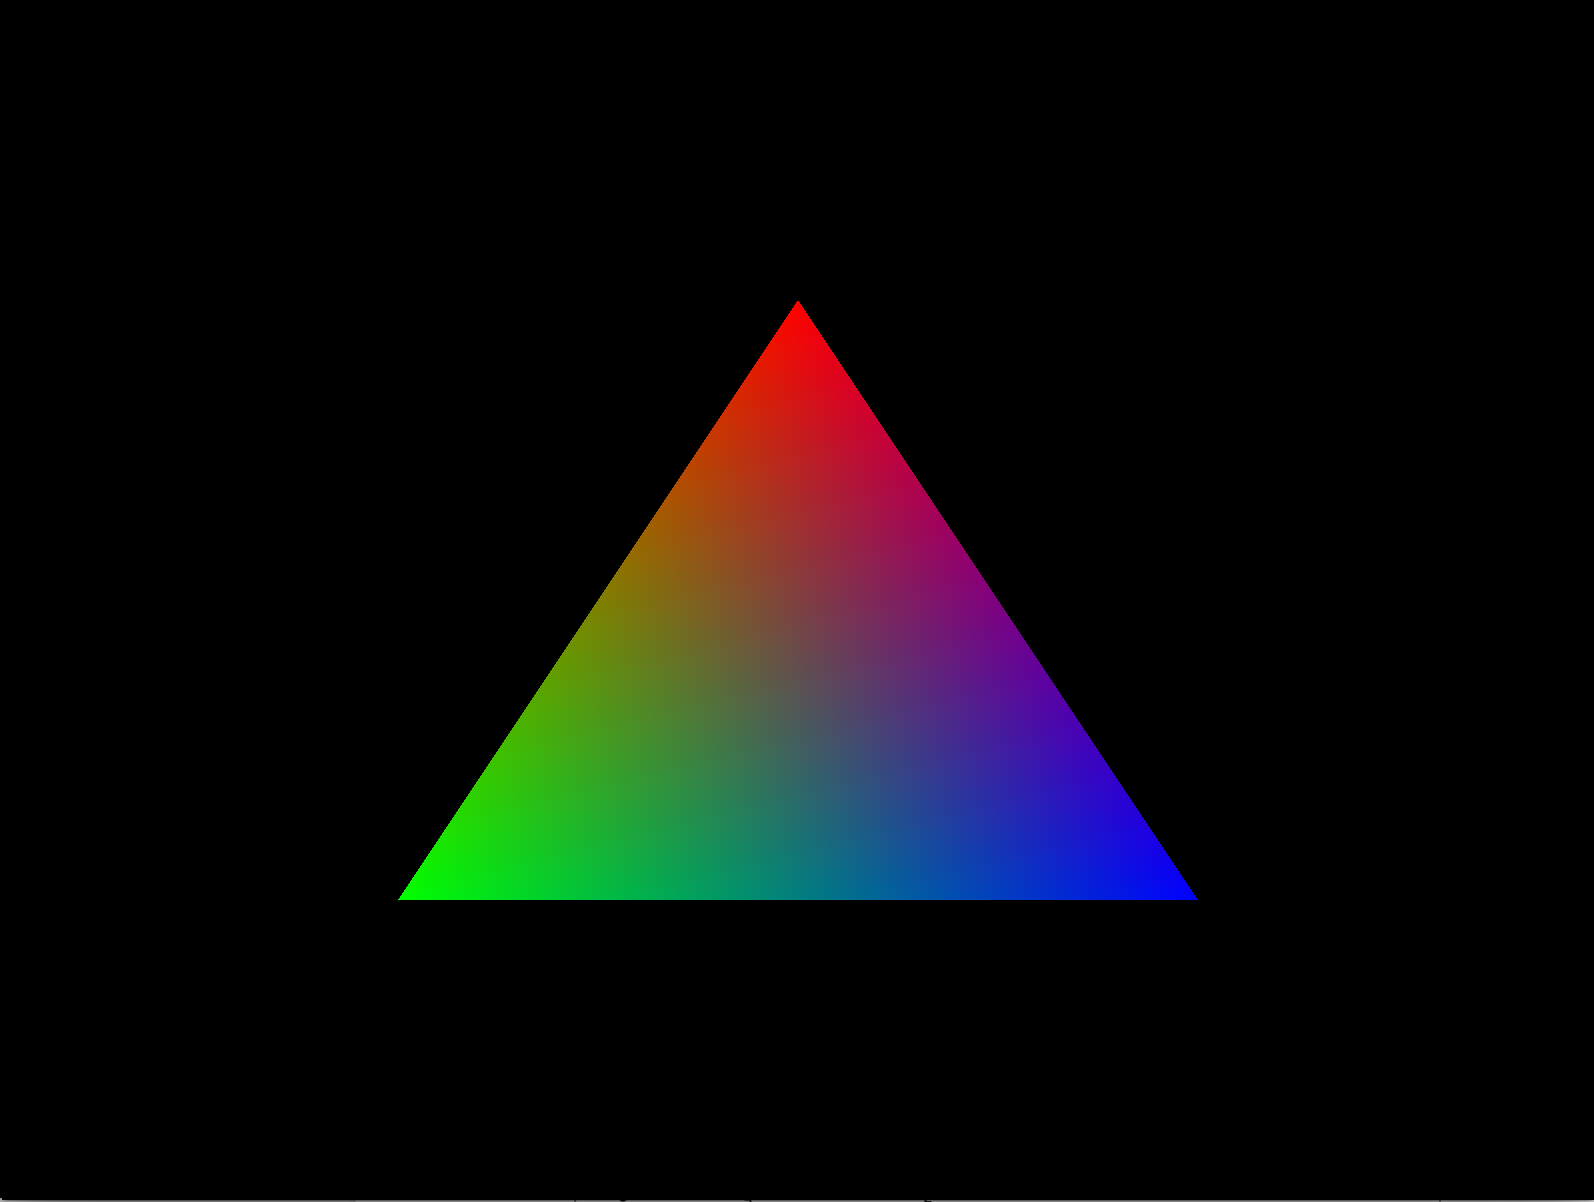
\includegraphics[width=\linewidth]{interpolation.png}
    \caption{Interpolation.}\label{fig:interpolation}
  \endminipage\hfill
  \minipage{0.32\textwidth}
    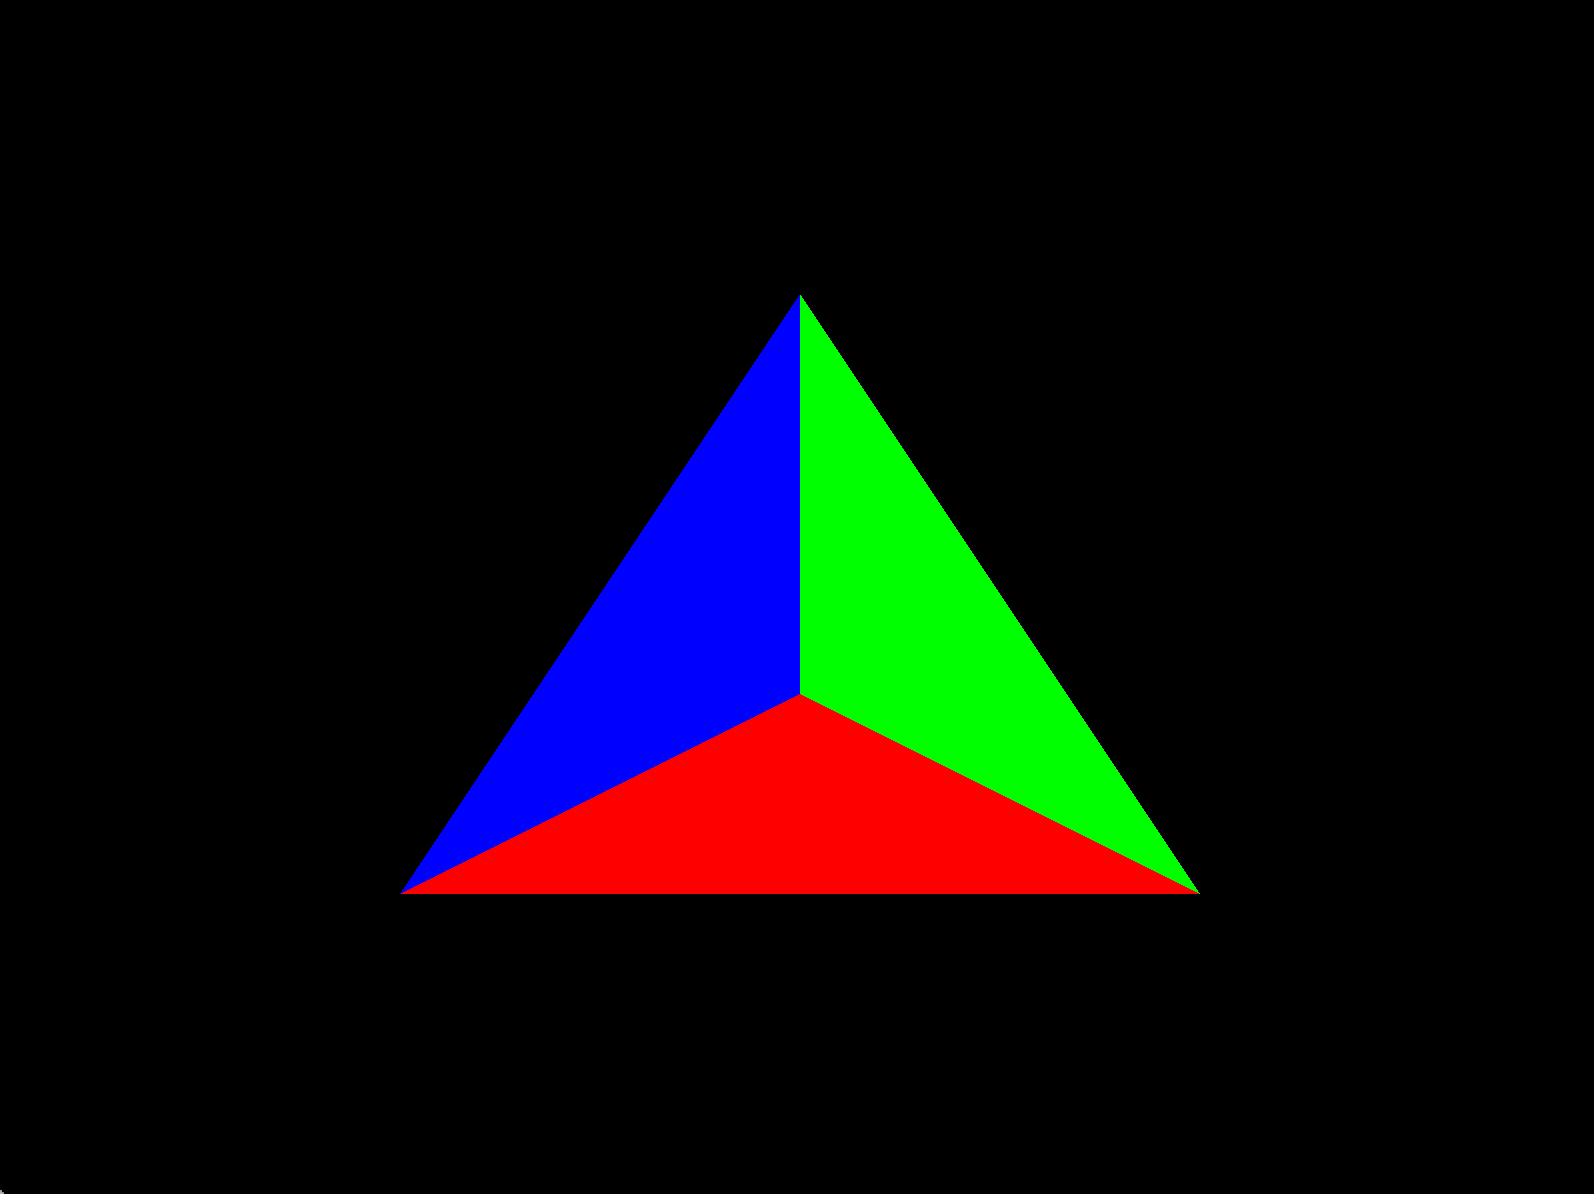
\includegraphics[width=\linewidth]{min.png}
    \caption{Min Diagram.}\label{fig:min}
  \endminipage\hfill
  \minipage{0.32\textwidth}%
    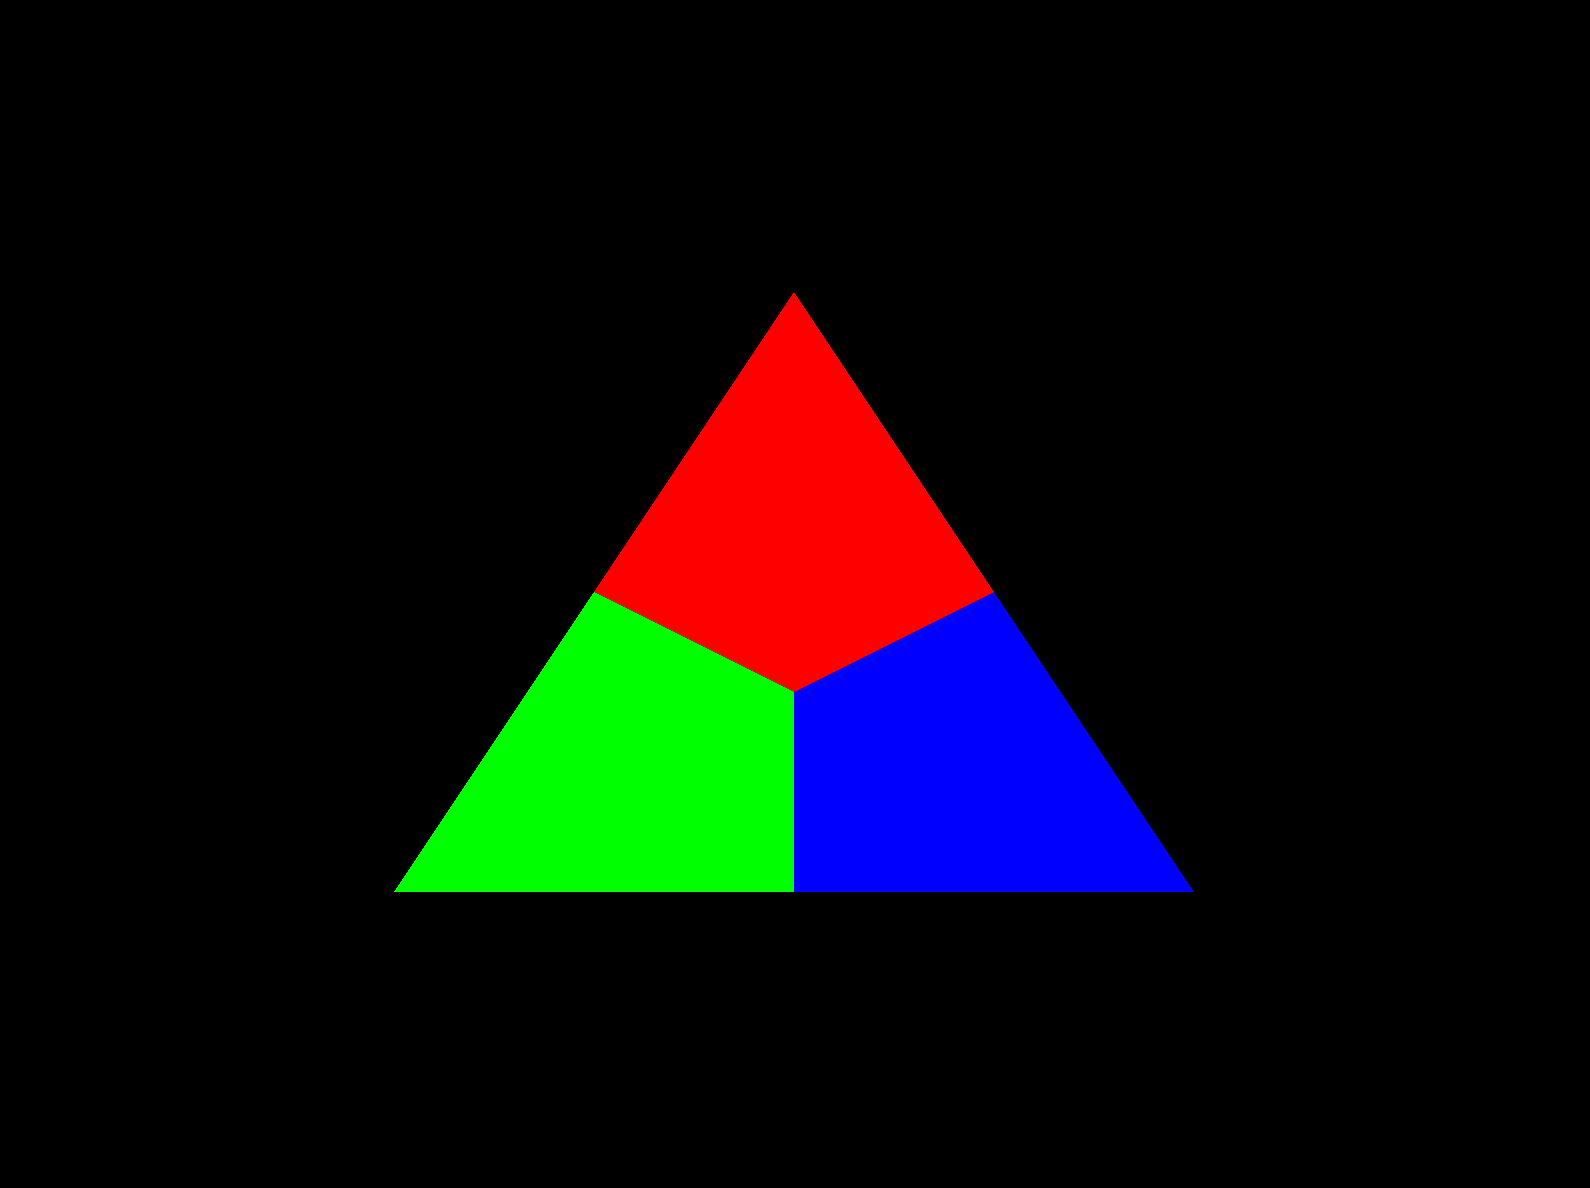
\includegraphics[width=\linewidth]{max.png}
    \caption{Max Diagram.}\label{fig:max}
  \endminipage
  \end{figure}

Some achievable approaches can make out focusing on the distance from vertices. Undoubtedly for each vertex, we can recognize some closer points to it and some not.
One approach can be represented by the following. 

Let's consider a triangle in which in the top vertex we have the red 
color, bottom left the green and in the bottom right the blue.
The triangle 
barycentre divides
each median into two pieces that have a 2:1 ratio.
In fig.\ref{fig:min} the farthest region from a vertex is colored. Also, we can notice that regions are divided by the "longer" part of medians.
In fig.\ref{fig:max} we have colored the closest region from a vertex. 
These approaches can be expressed in relation to barycentric coordinates.
\newgeometry{paper=a4paper,margin=1.65in}

\section{Project description and Goals}
Alternative data visualization techniques can be found using the power of barycentric coordinates and GPU programming.
The usual way to visualize data for a triangle mesh is to associate data 
to vertices and then interpolating over the mesh triangles, that does not work in case of edges and triangles. 


As a \textbf{first main goal}, we want to expand the idea of \textit{Flat Shading}\footnote{Flat Shading: the idea is to draw all the pixels
of a triangle with the same 
color.} also on vertices and edges. A next step could be to split the surface of triangle meshes into regions around vertex (fig.\ref{fig:left}) and edges (fig.\ref{fig:right}) and 
color them. 

\begin{figure}[!htb]
\minipage{0.45\textwidth}
  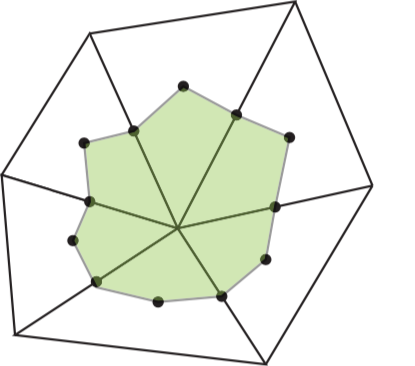
\includegraphics[width=\linewidth]{left.png}
  \caption{Region around a vertex.}\label{fig:left}
\endminipage\hfill
\minipage{0.45\textwidth}
  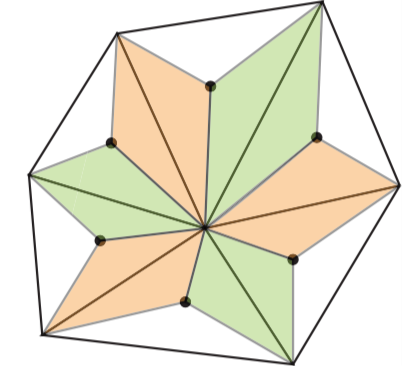
\includegraphics[width=\linewidth]{right.png}
  \caption{Region around an edge.}\label{fig:right}
\endminipage
\end{figure}
These regions can be determined using barycentric coordinates and GPU fragment program. 
Visualizing data given at the vertices or edges of the mesh in a piecewise constant simulates the classical triangle flat shading.

Examples of these edge and vertex data are the discrete Gaussian and discrete mean value curvature.

The next step will be to analyze the results obtained. A \textbf{second main goal} would be to extend the project set up a \textit{Gouraud Shading}\footnote{Gouraud Shading: linear interpolate data given at the vertices over the triangles of the mesh, resulting in a piecewise linear and continuous visualization of the data.}
for these new mesh tessellations. Using the barycentric coordinates and the fragment shader we can spell out a similar piecewise linear continuous interpolation over vertex and edge of regions (fig.\ref{fig:left} and fig.\ref{fig:right}).
The final step would be to evaluate these data.

\section{Milestones and Project Timeline} 
\subsection{Milestones}
\begin{itemize}
\item [\textbf{M1)}] Environment setup.
\item [\textbf{M2)}] Flat shading on vertices and edges.
\item [\textbf{M3)}] GPU fragment program.
\item [\textbf{M4)}] Extension of Gouraud shading.
\item [\textbf{M5)}] Project thesis and report.
\end{itemize}

\subsection{Tasks}
\begin{itemize}
  \item [\textbf{T1)}] GPU vertex program.
  \item [\textbf{T2)}] Extend Flat Shading.
  \item [\textbf{T3)}] Split surface triangle mesh into regions.
  \item [\textbf{T4)}] GPU fragment program.
  \item [\textbf{T5)}] Evaluation and comparison.
  \item [\textbf{T6)}] Extend Gouraud Shading.
  \item [\textbf{T7)}] Evaluation and comparison.
  \item [\textbf{T8)}] Project thesis and report.
  \end{itemize}

  \noindent\resizebox{\textwidth}{!}{
    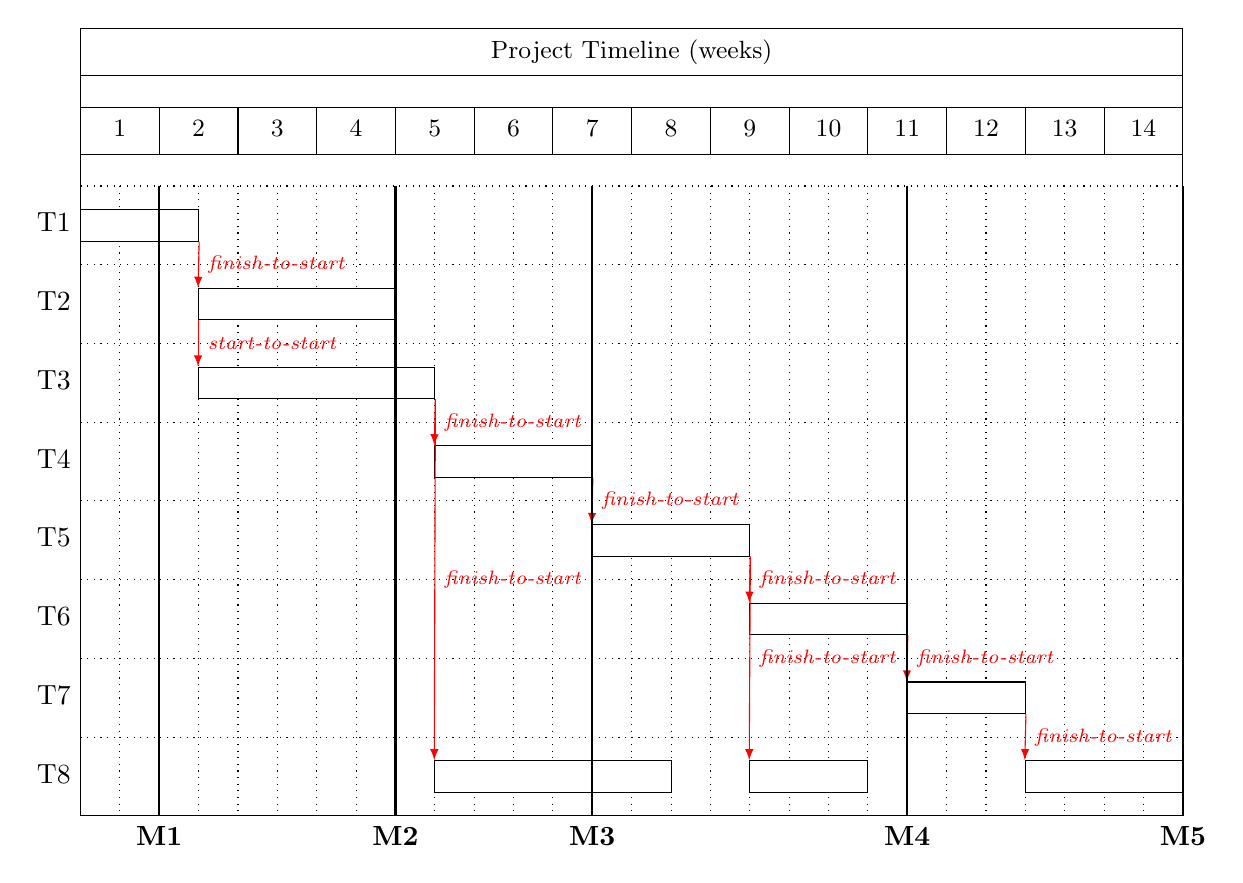
\begin{tikzpicture}
\begin{ganttchart}[vgrid, hgrid, link/.style={-latex, red},vrule/.style={thick, black},
  vrule label font=\bfseries]{1}{28}
  \gantttitle{Project Timeline (weeks)}{28} \\
  \gantttitlelist{1,...,14}{2} \\
  \ganttbar{T1}{1}{3} \\
  \ganttbar{T2}{4}{8} \ganttnewline
  \ganttbar{T3}{4}{9} \ganttnewline
  \ganttbar{T4}{10}{13} \ganttnewline
  \ganttbar{T5}{14}{17} \ganttnewline
  \ganttbar{T6}{18}{21} \ganttnewline
  \ganttbar{T7}{22}{24} \ganttnewline
  \ganttbar{T8}{18}{20}
  \ganttbar{}{10}{15}
  \ganttbar{}{25}{28}
  \ganttlink[link type=f-s]{elem0}{elem1}
  \ganttlink[link type=s-s]{elem1}{elem2}
  \ganttlink[link type=f-s]{elem2}{elem3}
  \ganttlink[link type=f-s]{elem3}{elem4}
  \ganttlink[link type=f-s]{elem4}{elem5}
  \ganttlink[link type=f-s]{elem5}{elem6}
  \ganttlink[link type=f-s]{elem4}{elem7}  
  \ganttlink[link type=f-s]{elem2}{elem8}
  \ganttlink[link type=f-s]{elem6}{elem9}
  \ganttvrule{M1}{2}
  \ganttvrule{M2}{8}
  \ganttvrule{M3}{13}
  \ganttvrule{M4}{21}
  \ganttvrule{M5}{28}
\end{ganttchart}
\end{tikzpicture}}

\end{document}  

